\section{Challenges and Limitations}\label{sec:challenges}

After preprocessing the Mapillary Vistas dataset, we faced some challenges that are worth mentioning. For instance, we created a script that displays images from the dataset and draws their respective bounding boxes in case billboards are present. We noticed that in some images, billboards were not selected, while in others, letters representing the names of buildings were incorrectly classified as billboards. This can be seen in more detail in figure 2.1.\\

This misclassification might be due to the fact that the authors and those responsible for annotating the original dataset did not explicitly focus on billboards, even though the "billboard" class is part of the original set of classes in the dataset. We believe this could become a limitation when training the object detector and, eventually, impact its accuracy. This will be discussed again in the results section.

\begin{figure}[H]
    \centering
    % First image
    \begin{subfigure}[b]{0.45\textwidth}
        \centering
        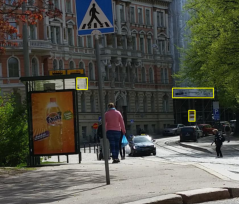
\includegraphics[width=\textwidth]{src/images/mis1.png}
        \caption{Billboard not selected}
        \label{fig:image1}
    \end{subfigure}
    \hfill
    % Second image
    \begin{subfigure}[b]{0.45\textwidth}
        \centering
        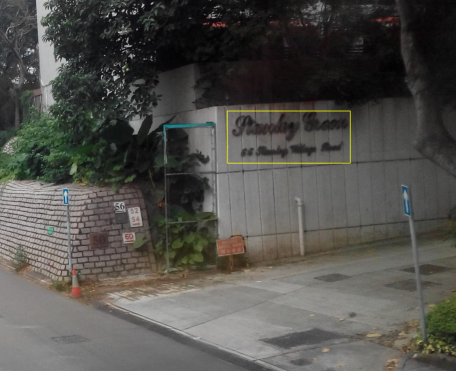
\includegraphics[width=\textwidth]{src/images/mis2.png}
        \caption{Miscslassification example}
        \label{fig:image2}
    \end{subfigure}
    \caption{Examples of a billboard not being classified (left) and a misclassification case in the training set of the Mapillary Vistas dataset.}
    \label{fig:comparison}
\end{figure}


